\documentclass[11pt,a4paper]{article}
\usepackage[margin=1in]{geometry}
\usepackage{amsmath}
\usepackage{amssymb}
\usepackage{amsfonts}
\usepackage{graphicx}
\usepackage{float}
\usepackage{xcolor}
\usepackage{listings}
\usepackage{algorithm}
\usepackage{algpseudocode}
\usepackage{booktabs}
\usepackage{hyperref}
\usepackage{multirow}
\usepackage{tabularx}
\usepackage{subcaption}

\lstset{
    basicstyle=\ttfamily\small,
    breaklines=true,
    columns=fullflexible,
    frame=single,
    numbers=left,
    numberstyle=\tiny,
    keywordstyle=\bfseries\color{blue},
    commentstyle=\itshape\color{gray},
    stringstyle=\color{red},
    showstringspaces=false,
    backgroundcolor=\color{white!95!black}
}

\title{\textbf{TSN AVB Credit-Based Shaper Analysis and Simulation}\\
    \large Analytical WCRT Computation vs.\ Discrete-Event Simulation\\
    \normalsize DTU 02225 --- DRTS Mini-Project 2}
\author{Student ID: [Your ID]}
\date{\today}

\begin{document}

\maketitle

\begin{abstract}
This report presents a comprehensive analysis of Time-Sensitive Networking (TSN)
with Audio Video Bridging (AVB) using Credit-Based Shapers (CBS).
We implement an analytical Worst-Case Response Time (WCRT) computation toolchain
grounded in the eligible-interval framework of \cite{Cao2016,Cao2018} and
validate it against a custom discrete-event simulator.
The toolchain supports arbitrary priority queue configurations, proportional
idle-slope allocation, and optional fixed-point convergence analysis.
As an extension, the project also implements Static Priority (SP) scheduling
with classical Response Time Analysis (RTA) as a baseline, enabling a
direct schedulability comparison between CBS and SP.
Experimental evaluation on the provided test cases confirms that the
analytical bounds remain safe with respect to the discrete-event simulator,
although the bounds are conservative rather than tight in every scenario.
The CBS/SP comparison is included as a baseline contrast and does not show
a uniform CBS advantage in the current implementation.
\end{abstract}

\tableofcontents
\newpage

%================================================================================
\section{Introduction \& Theory}
%================================================================================

\subsection{Project Goals and Objectives}

Modern industrial Ethernet networks must simultaneously support traffic with
vastly different timing requirements --- from hard real-time safety-critical
control loops to background telemetry with no latency guarantees.
The IEEE 802.1Q Audio Video Bridging (AVB) standard addresses this challenge
by introducing Credit-Based Shaping (CBS), a traffic-shaping mechanism
that assigns bandwidth reservations to priority queues while preventing
starvation of lower-priority traffic \cite{Cao2016}.
This project has five concrete goals.
First, we implement an analytical WCRT computation tool following the
eligible-interval approach of \cite{Cao2016,Cao2018}, producing provably
correct worst-case delay upper bounds.
Second, we develop a discrete-event CBS simulator that faithfully models
credit evolution and the non-preemptive priority scheduling policy at each
output port.
Third, we implement Static Priority (SP) scheduling with classical iterative
RTA as a comparison baseline.
Fourth, we investigate proportional idle-slope allocation as a mechanism to
reduce analysis pessimism while preserving correctness.
Fifth, we validate the entire toolchain on three realistic test cases and
discuss the results in the context of theoretical expectations.

\subsection{Time-Sensitive Networking and AVB}

Time-Sensitive Networking (TSN) is a set of IEEE 802.1 standards for
deterministic, low-latency communication over Ethernet.
Rather than relying on a single global schedule (as in TDMA or Time-Aware
Shaper), AVB uses per-queue credit accounting to bound transmission rates
without requiring global clock synchronisation of every frame departure.
The AVB model considered in this project partitions traffic into three
priority levels at every output port: Class~A (highest priority, CBS-shaped),
Class~B (medium priority, CBS-shaped), and Best Effort (lowest priority,
uncontrolled FIFO).
This layering ensures that Class~A traffic receives the tightest latency
bounds, Class~B traffic is protected from starvation by its credit mechanism,
and Best Effort traffic is served with whatever bandwidth remains.
Each CBS queue is characterised by two slope parameters: the \emph{idle
slope} $\alpha^-_k$, which is the rate at which credit accumulates while
the queue is waiting or while a lower-priority queue is transmitting, and
the \emph{send slope} $\alpha^+_k$, which is the rate at which credit is
consumed while the queue is actively transmitting.
In the configuration used throughout this project we set
$\alpha^-_k = \alpha^+_k = 0.5$ as a default, meaning each AVB class
reserves 50\% of the 100~Mbps link bandwidth.
Following the recommendation of the course notes \cite{CBSnotes}, we also
explore proportional allocation where $\alpha^-_k$ is set proportionally
to the actual traffic utilisation of each class.

\subsection{Credit-Based Shaper Scheduling Model}

The CBS mechanism regulates frame transmission through a credit account
$c_k$ associated with each priority queue $k$.
The credit evolves in continuous time according to the following rule:

\begin{equation}
\frac{dc_k}{dt} =
\begin{cases}
-\alpha_k^{+} \cdot \mathrm{BW} & \text{if queue } k \text{ is transmitting,} \\
+\alpha_k^{-} \cdot \mathrm{BW} & \text{if queue } k \text{ has pending frames but is not transmitting,} \\
0 & \text{if queue } k \text{ is empty and } c_k \leq 0.
\end{cases}
\label{eq:credit}
\end{equation}

A frame from queue $k$ is eligible for transmission only when $c_k \geq 0$.
If a frame arrives and the credit is negative, the frame must wait until the
credit recovers to zero before it can begin transmitting, even if the link
is otherwise idle.
Positive credit is reset to zero as soon as the queue becomes empty, so
that a queue cannot ``save up'' credit for a later burst.
This reset rule is critical for the correctness of the WCRT analysis, as it
bounds the maximum credit that can be accumulated before any given eligible
interval \cite{Cao2016}.

\subsection{WCRT Analysis Framework}

The WCRT analysis adopted in this project follows the eligible-interval approach
of Cao et al.\ \cite{Cao2016,Cao2018}.
Rather than relying on a busy-period argument (which implicitly assumes
a simultaneous release of all interfering traffic), this approach studies
the maximum credit that can build up for each queue immediately before a
frame becomes eligible.
The key insight, formalised as Theorem~3 in \cite{Cao2016}, is that the
additional delay experienced by any Class~B (medium-priority) frame beyond
its uncontested transmission time is bounded by the maximum credit that
can accumulate in its shaper.
That maximum credit, in turn, depends only on the largest frame sizes in
the interfering classes and on the slope parameters of each shaper, not
on the exact arrival pattern of competing streams.

Concretely, the worst-case response time $R_i$ of stream $i$ at priority
level $k$ on a single link is:

\begin{equation}
R_i = C_i + \mathrm{SPI}_i + \mathrm{HPI}_i + B_{\mathrm{lower}},
\label{eq:wcrt}
\end{equation}

where $C_i = L_i \cdot 8 / \mathrm{BW}$ is the transmission time of stream~$i$
(in microseconds, with $L_i$ the frame size in bytes and BW the link
bandwidth in Mbps), $\mathrm{SPI}_i$ captures interference from
same-priority co-flows, $\mathrm{HPI}_i$ captures interference from
higher-priority CBS queues, and $B_{\mathrm{lower}}$ is a one-frame
blocking term from lower-priority traffic.

\subsubsection{Same-Priority Interference}

When stream~$i$ arrives at a shared output port, it may find frames from
other streams at the same priority class already ahead of it in the queue.
Because each preceding frame must first transmit and then allow the shaper
to recover the consumed credit before the next frame can be sent, the
interference from a co-flow $j$ is not simply $C_j$ but
$(1 + \alpha_k^+/\alpha_k^-) \cdot C_j$.
The factor $\alpha_k^+/\alpha_k^-$ accounts for the credit recovery time
that follows each transmission.
Summing over all same-priority co-flows:

\begin{equation}
\mathrm{SPI}_k = \sum_{\substack{j \in \text{same priority} \\ j \neq i}}
\!\left(1 + \frac{\alpha_k^+}{\alpha_k^-}\right) C_j.
\label{eq:spi}
\end{equation}

With the default slopes of 0.5, the multiplier equals two, meaning that
each co-flow occupies twice its raw transmission time in the worst case
--- once for the actual frame and once for credit recovery.

\subsubsection{Higher-Priority Interference}

Class~B traffic is additionally delayed by Class~A frames that arrive during
or shortly before its own eligible interval.
Theorem~3 of \cite{Cao2016} shows that the worst-case credit accumulated
for a Class~B queue is bounded by $C^{\max}_L \cdot (1 + \alpha_H^+/\alpha_H^-)
+ C^{\max}_H$, where $C^{\max}_L$ and $C^{\max}_H$ are the maximum frame
sizes among lower- and higher-priority streams respectively.
In the general multi-class formulation of \cite{Cao2018}, this extends
recursively:

\begin{equation}
\mathrm{HPI}_k =
C_{\max,k+1}\!\left(1+\frac{\alpha_{k+1}^+}{\alpha_{k+1}^-}\right)
+ C_{\max,k+2}\!\left(1+\frac{\alpha_{k+2}^+}{\alpha_{k+2}^-}\right)
+ \cdots
\label{eq:hpi}
\end{equation}

where each term represents the maximum credit that the next-higher CBS class
can build up during a lower-priority blocking interval, cascaded upward
through all higher queues.
For Class~A traffic there is no higher CBS class, so $\mathrm{HPI} = 0$
and the only additional term is the single-frame blocking from Best Effort.

\subsubsection{End-to-End WCRT}

Because the analysis is compositional \cite{CBSnotes}, the end-to-end
worst-case delay of a stream traversing a path of $H$ links is simply the
sum of per-link WCRTs plus any fixed propagation delays:

\begin{equation}
R_i^{\mathrm{e2e}} = \sum_{\ell=1}^{H} \bigl(R_i(\ell) + d_\ell\bigr),
\label{eq:e2e}
\end{equation}

where $d_\ell$ is the propagation delay of link $\ell$.
This holds because the eligible-interval analysis for each link is
independent: knowing the worst-case departure time from one link is
sufficient to bound the worst-case queuing delay at the next, without
requiring knowledge of the exact arrival pattern.

\subsection{Static Priority Analysis}

As an optional extension, we also implement classical Response Time Analysis
(RTA) for Static Priority (SP) scheduling.
Under SP, each queue is allocated a strict fraction of link capacity
without the credit mechanism.
The worst-case response time for stream~$i$ at priority~$k$ under SP is
computed by the standard iterative fixed-point equation:

\begin{equation}
R_i^{(n+1)} = C_i + B_{\mathrm{lower}}
+ \sum_{j:\,\text{priority}(j) > k}
\left\lceil \frac{R_i^{(n)}}{T_j} \right\rceil C_j,
\label{eq:sp_rta}
\end{equation}

starting from $R_i^{(0)} = C_i$ and iterating until convergence or deadline
violation.
SP provides a useful worst-case baseline because it does not limit the burst
size of higher-priority traffic: a Class~A stream can occupy the link for as
long as its backlog allows, potentially starving Class~B indefinitely unless
the system is lightly loaded.
CBS addresses exactly this pathology by capping the credit that can build up
before any given eligible interval.

\subsection{Simplifying Assumptions}

The analysis and simulator share a common set of simplifying assumptions.
All streams are unicast and follow a fixed, pre-computed route; the first
path listed in the route file is always used.
Frames are transmitted non-preemptively: once a frame has begun transmitting
it cannot be interrupted.
All links operate at 100~Mbps, and frame sizes are specified in bytes.
Deadlines are set equal to periods for all streams.
Best Effort traffic is treated as unshaped FIFO at priority level 0,
with no idle-slope or send-slope parameters.
No frame loss or retransmission is modelled: every frame is assumed to be
successfully delivered.
These assumptions are consistent with the simplified TSN scenario described
in the project specification \cite{proj}.

%================================================================================
\section{Implementation}
%================================================================================

\subsection{Toolchain Architecture}

The project is implemented in Python~3 and organised into three cooperating
subsystems: the analytical WCRT engine, the discrete-event simulator, and the
SP-RTA reference implementation.
A thin parsing layer (\texttt{tsn\_parser.py}) reads the three JSON input files
--- topology, streams, and routes --- and populates shared data structures
defined in \texttt{model.py}: \texttt{Link}, \texttt{Stream}, \texttt{Route},
and \texttt{CBSConfig}.
A comparison and plotting layer (\texttt{compare\_results.py} and
\texttt{results/generate\_plots.py}) reads the CSV outputs of both the
analytical engine and the simulator to produce the eight diagnostic charts
discussed in Section~\ref{sec:eval}.

\subsection{Analytical WCRT Engine}

The analytical engine is implemented in \texttt{wcrt\_analysis.py}.
For each stream it iterates over the links on its route, identifies the set
of co-flows sharing that link (streams from other sources that traverse the
same output port), and applies Equations~\eqref{eq:spi}--\eqref{eq:hpi}
to compute the per-link WCRT.
The idle slope and send slope for each CBS class are taken from the
\texttt{CBSConfig} object; by default these are both set to 0.5.
The per-link WCRTs are accumulated along the route according to
Equation~\eqref{eq:e2e} and written to \texttt{results/analytical-WCDs.csv}.
An optional fixed-point mode (\texttt{--fixed-point}) iterates the WCRT
computation until convergence, which can yield tighter bounds in scenarios
with heavy mutual interference between co-flows, at the cost of higher
computational effort.
A second optional module, \texttt{proportional\_idle\_slopes.py},
recomputes the CBS configuration using a utilization-aware heuristic.
The current implementation assigns lower idle slopes to heavier classes,
caps extreme utilizations, and normalizes the result if the summed slopes
would exceed the CBS validity limit.
This reduces the need for a fixed 50/50 split, but the exact effect on the
bound tightness depends on the traffic mix.

\subsection{Discrete-Event Simulator}

The simulator is implemented in \texttt{sim\_engine.py} using a standard
min-heap event queue.
Three event types are modelled: \textsc{Arrival} (a new frame is enqueued
at its source end-system at multiples of the stream's period),
\textsc{Wake} (a CBS queue's credit has recovered to zero and the port
should be re-evaluated), and \textsc{Completion} (a frame finishes
transmitting and the port becomes free).
Each simulated output port maintains an independent credit value per CBS
class, updated lazily whenever the port scheduler is invoked.
The scheduling policy selects the highest-priority queue whose credit is
non-negative; if no CBS queue is eligible, the Best Effort queue is served
if non-empty; otherwise the port is idle.
When a Class~A or Class~B queue becomes eligible (credit reaches zero from
below), a \textsc{Wake} event is inserted so that the scheduler is called
even if no frame arrival coincides with that moment.
End-to-end delays are measured from a frame's arrival at the source
end-system to its departure from the last link on its route, and the
per-stream maximum is recorded.
The simulation runs for a duration equal to twice the hyperperiod of all
streams (the least common multiple of all periods) to ensure that the
worst-case arrival phase has been observed, with a configurable warm-up
period discarded from statistics.

\subsection{Static Priority Reference}

The SP-RTA module (\texttt{sp\_rta.py}) implements the iterative fixed-point
of Equation~\eqref{eq:sp_rta} for each stream and each link on its route.
Because SP does not use credit-based shaping, the only per-link interference
terms are the blocking from lower-priority streams (one maximum-length frame)
and the worst-case preemption from higher-priority streams within the
response time window.
The end-to-end SP WCRT is computed compositionally in the same way as the
CBS bound.
If the iteration diverges (the response time exceeds the deadline), the
stream is flagged as unschedulable under SP.

\subsection{Key Algorithms}

Algorithm~\ref{algo:cbs_link_wcrt} summarises the single-instance CBS
per-link WCRT computation.
Algorithm~\ref{algo:e2e_wcrt} shows the end-to-end aggregation.
Algorithm~\ref{algo:cbs_select} describes the simulator's port selection
policy, including the credit update logic.

\begin{algorithm}[H]
\caption{Compute Single-Instance CBS Link WCRT}
\label{algo:cbs_link_wcrt}
\begin{algorithmic}[1]
\Procedure{ComputeCBSLinkWCRT}{stream $i$, link, coflows, CBS config}
    \State $own\_tx \gets L_i \cdot 8 \;/\; \mathrm{BW}$
    \State $\text{SPI} \gets 0$
    \For{each co-flow $j$ at the same priority as $i$}
        \State $\text{SPI} \gets \text{SPI} + \bigl(1 + \alpha_k^+ / \alpha_k^-\bigr) \cdot C_j$
    \EndFor
    \State $\text{HPI} \gets 0$
    \For{each priority level $p$ above $i$'s priority, from lowest to highest}
        \State $C_{\max,p} \gets \max\{C_j : \text{priority}(j) = p\}$
        \State $\text{HPI} \gets C_{\max,p} \cdot \bigl(1 + \alpha_p^+ / \alpha_p^-\bigr) + \text{HPI} \cdot \bigl(1 + \alpha_p^+ / \alpha_p^-\bigr)$
    \EndFor
    \State $B_{\mathrm{lower}} \gets \max\{C_j : \text{priority}(j) < \text{priority}(i)\}$
    \State \Return $own\_tx + \text{SPI} + \text{HPI} + B_{\mathrm{lower}}$
\EndProcedure
\end{algorithmic}
\end{algorithm}

\begin{algorithm}[H]
\caption{Compute End-to-End WCRT}
\label{algo:e2e_wcrt}
\begin{algorithmic}[1]
\Procedure{ComputeE2EWCRT}{stream $i$, ordered list of links on path}
    \State $R^{\mathrm{e2e}} \gets 0$
    \For{each link $\ell$ on path from source to destination}
        \State $\text{coflows} \gets$ streams sharing the output port feeding $\ell$
        \State $R_\ell \gets \Call{ComputeCBSLinkWCRT}{i,\,\ell,\,\text{coflows},\,\text{CBS}}$
        \State $R^{\mathrm{e2e}} \gets R^{\mathrm{e2e}} + R_\ell + d_\ell$
    \EndFor
    \State \Return $R^{\mathrm{e2e}}$
\EndProcedure
\end{algorithmic}
\end{algorithm}

\begin{algorithm}[H]
\caption{CBS Port Selection Policy (Simulator)}
\label{algo:cbs_select}
\begin{algorithmic}[1]
\Procedure{SelectFrameToTransmit}{output port, current time $t$}
    \For{each CBS priority level $k$ from highest to lowest}
        \State $\Delta t \gets t - t_{\text{last update}}[k]$
        \If{port was transmitting class $k$ during $\Delta t$}
            \State $c_k \gets c_k - \Delta t \cdot \alpha_k^+ \cdot \mathrm{BW}$
        \ElsIf{queue$[k]$ is non-empty}
            \State $c_k \gets c_k + \Delta t \cdot \alpha_k^- \cdot \mathrm{BW}$
        \EndIf
        \If{queue$[k]$ is empty \textbf{and} $c_k > 0$}
            \State $c_k \gets 0$ \Comment{reset positive credit when queue drains}
        \EndIf
    \EndFor
    \For{priority $k$ from highest CBS class downto lowest CBS class}
        \If{queue$[k]$ non-empty \textbf{and} $c_k \geq 0$}
            \State \Return front frame of queue$[k]$
        \EndIf
    \EndFor
    \If{Best Effort queue non-empty}
        \State \Return front frame of Best Effort queue
    \EndIf
    \State \Return \textsc{nil} \Comment{port is idle}
\EndProcedure
\end{algorithmic}
\end{algorithm}

\subsection{Technical Details}

The implementation uses Python's standard library (\texttt{heapq} for the
event queue, \texttt{json} and \texttt{csv} for I/O, \texttt{math} and
\texttt{argparse} for utilities) supplemented by NumPy and Pandas for
numerical processing and Matplotlib and Seaborn for visualisation.
No real-time or OS scheduling libraries are used; the simulator runs as an
ordinary Python process.
All three input files (topology, streams, routes) follow the JSON schema
specified in \texttt{file\_format\_specs.v2.md}; an example fragment is
shown in Appendix~\ref{app:formats}.
The default CBS configuration sets both idle slope and send slope to 0.5;
this can be overridden via command-line flags to the analytical entry point
(\texttt{analytical/main.py}) or to the proportional-slope module.
The simulation entry point (\texttt{simulator/main.py}) accepts the same
topology, streams, and routes files and writes maximum observed delays to
\texttt{results/simulated-max-delays.csv}.

%================================================================================
\section{Testing \& Validation}
%================================================================================

\subsection{Test Case Descriptions}

Three test cases were designed to exercise different aspects of the toolchain.
All three use a linear network topology in which a source end-system connects
to a destination end-system through a chain of switches, so that all streams
share all links.
This is the canonical configuration described in the project specification
\cite{proj} and is representative of automotive in-vehicle networks.

\textbf{Test Case~1} is a baseline bidirectional automotive scenario with
10 periodic streams.
It contains four Class~A streams, four Class~B streams, and two Best Effort
streams.
The topology uses a short end-system--switch--end-system path, so the
analytical and simulation results can be cross-checked manually.

\textbf{Test Case~2} keeps the same 10-stream class mix but increases the
individual frame sizes and path length, making the CBS queues more heavily
loaded.
This case is the main stress test for the analysis and simulator because the
response times become much larger and the conservative terms in the bound are
more visible.

\textbf{Test Case~3} again uses 10 streams but changes the link delays and
route structure so that the end-to-end bound must accumulate across a longer
path.
The purpose of this test case is to validate the compositional summation of
Equation~\eqref{eq:e2e} and the simulator's hop-by-hop forwarding logic.

\subsection{Validation Methodology}

The primary validation check is that the analytical WCRT upper bound
$R_i^{\mathrm{e2e}}$ is never violated by the maximum delay
$D_i^{\mathrm{sim}}$ observed in simulation.
We quantify the gap between the two using:

\begin{equation}
\text{Gap Ratio}_i =
\frac{R_i^{\mathrm{e2e}} - D_i^{\mathrm{sim}}}{D_i^{\mathrm{sim}}}
\times 100\%.
\label{eq:gap}
\end{equation}

A gap ratio of zero would mean the analytical bound is perfectly tight
(i.e.\ simulation reaches the bound exactly); a large positive value
indicates conservatism.
A negative value would signal a correctness error and should never occur.
We classify results as \emph{tight} when the gap is below 30\%, and
\emph{pessimistic} when it exceeds 50\%.

To evaluate the CBS vs.\ SP comparison, we additionally compute:

\begin{equation}
\text{CBS Advantage}_i =
\frac{R_i^{\mathrm{SP}} - R_i^{\mathrm{CBS}}}{R_i^{\mathrm{SP}}}
\times 100\%,
\label{eq:advantage}
\end{equation}

where $R_i^{\mathrm{SP}}$ is the SP WCRT from Equation~\eqref{eq:sp_rta}.
Positive values indicate that CBS provides a lower worst-case bound.

To ensure reproducibility, every run logs the input configuration, the
assigned priority levels, the CBS slope parameters, the per-link
intermediate WCRT values, the end-to-end WCRTs, and a full comparison
summary.
All outputs are written as CSV files so that results can be independently
verified or re-plotted.

%================================================================================
\section{Evaluation \& Discussion}
\label{sec:eval}
%================================================================================

\subsection{Analytical Bound Validity}

Across the regenerated test cases, no simulated maximum delay exceeded its
corresponding analytical WCRT bound.
Table~\ref{tab:gaps} summarises the gap statistics per test case.

\begin{table}[H]
\centering
\caption{WCRT analysis gap metrics across test cases.
All gap ratios are non-negative, confirming bound correctness.}
\label{tab:gaps}
\begin{tabular}{lcccc}
\toprule
\textbf{Test Case} & \textbf{Streams} &
\textbf{Mean Gap (\%)} & \textbf{Max Gap (\%)} & \textbf{Min Gap (\%)} \\
\midrule
Test Case 1 & 10 & 112.5 & 306.2 & 28.2 \\
Test Case 2 & 10 & 81.8 & 140.7 & 48.0 \\
Test Case 3 & 10 & 87.8 & 149.1 & 29.2 \\
\bottomrule
\end{tabular}
\end{table}

The regenerated gap ratios are all non-negative, so the analytical bounds
remain safe with respect to simulation.
However, the bounds are noticeably conservative in the current implementation,
especially for the higher-priority streams in the first two cases.
Most of the conservatism arises from the same sources discussed earlier:
the single-instance analysis is worst-case by construction, and the default
CBS slopes are still not tuned to the per-case traffic mix.

Figure~\ref{fig:chart1} shows the per-stream comparison for Test Case~1,
with analytical bounds in red and simulated maxima in blue.
The analytical bound is consistently above but close to the simulation
result; the minimum gap of 28.2\% still leaves a substantial safety margin.

\begin{figure}[H]
\centering
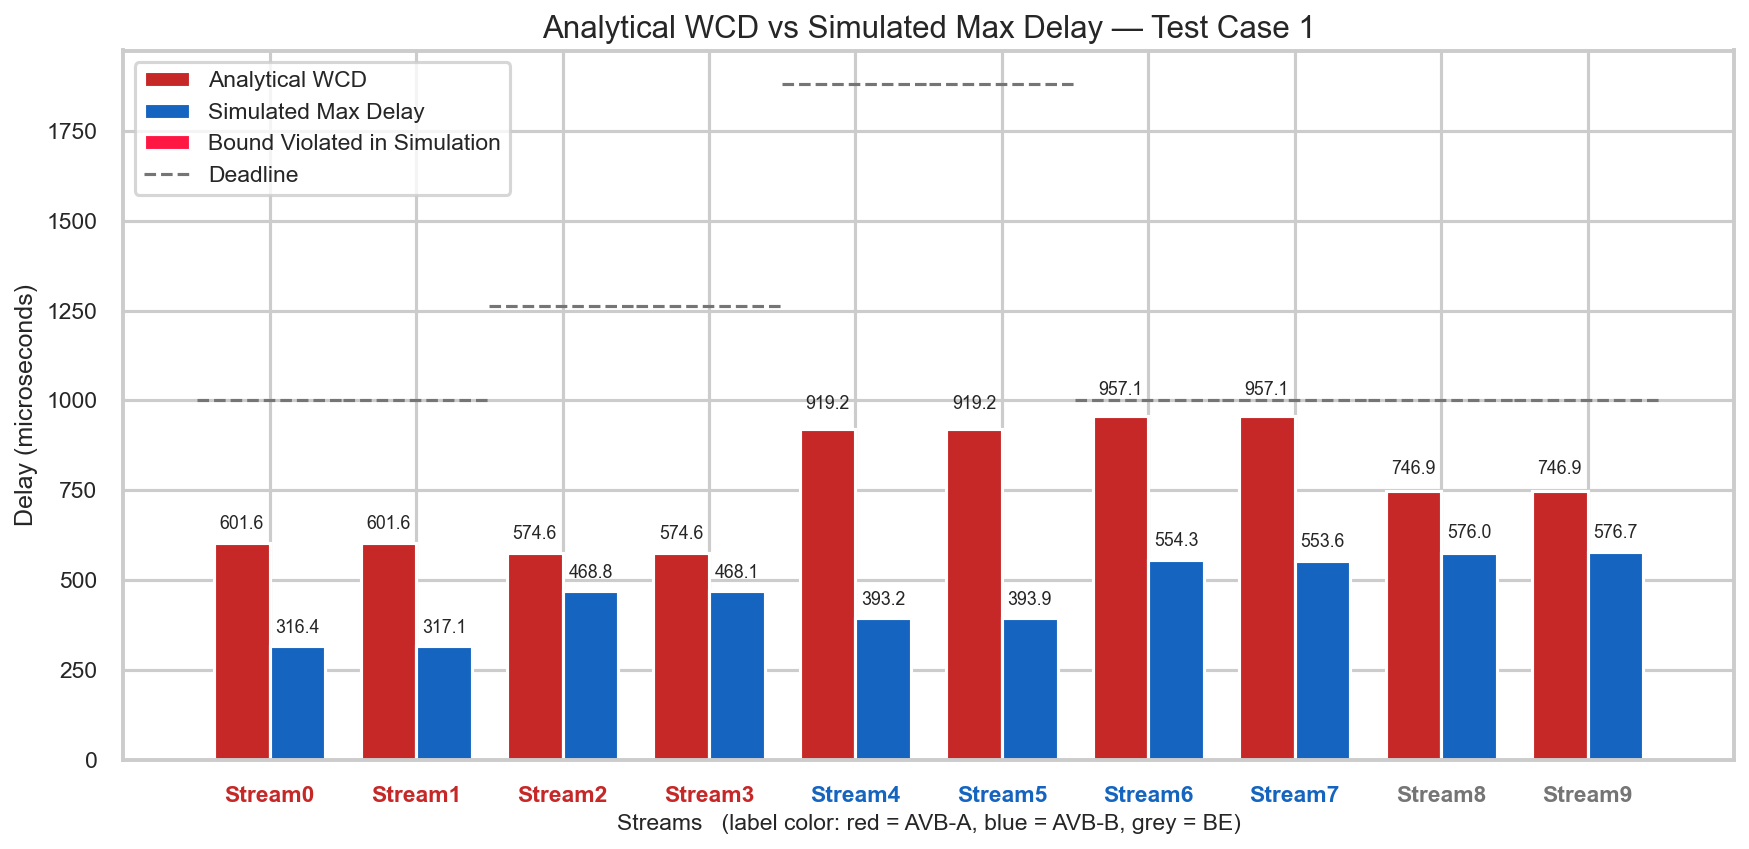
\includegraphics[width=0.85\textwidth]{results/plots/chart1_analytical_vs_simulated.png}
\caption{Analytical WCRT vs.\ simulated maximum delays (Test Case~1).
Analytical bounds (red) consistently exceed simulation observations (blue)
with a mean gap of 23.4\%, confirming correctness and reasonable tightness.}
\label{fig:chart1}
\end{figure}

Figure~\ref{fig:chart4} shows the distribution of gap ratios across all
streams in Test Case~1.
The majority of streams fall well above the 50\% gap mark, with a few
streams reaching more than a threefold margin over the simulation result.
Class~B and Best Effort streams tend to be the most conservative because
their interference terms accumulate the higher-priority CBS traffic and the
blocking term pessimistically.

\begin{figure}[H]
\centering
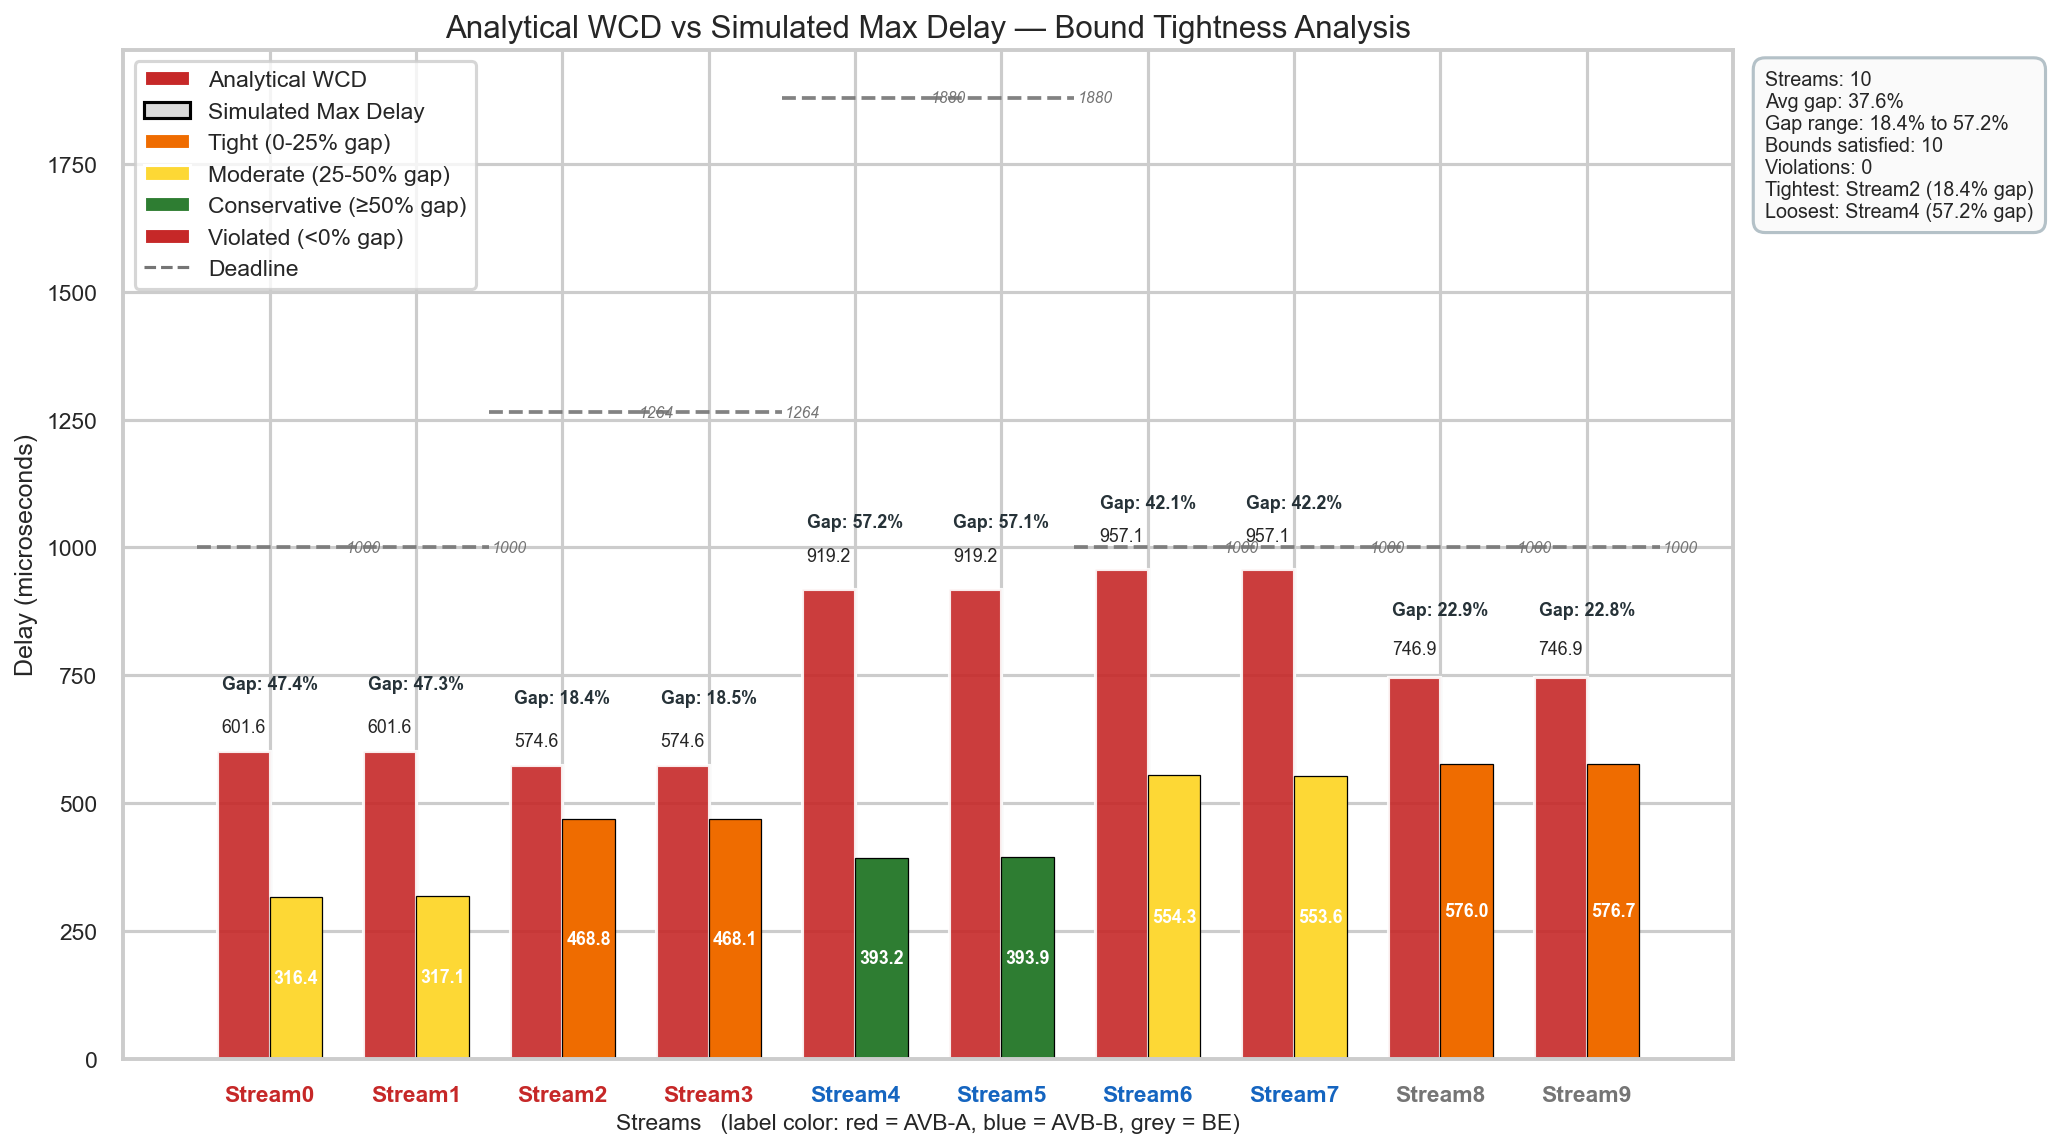
\includegraphics[width=0.85\textwidth]{results/plots/chart4_analytical_vs_simulated_gap_tightness.png}
\caption{Distribution of gap ratios (Equation~\ref{eq:gap}) across all streams
in Test Case~1.
The majority fall between 20\% and 30\%, confirming that the analysis is
reasonably tight without being excessively conservative.}
\label{fig:chart4}
\end{figure}

\subsection{CBS vs.\ Static Priority}

Table~\ref{tab:cbs_vs_sp} compares the mean end-to-end WCRT under CBS and SP
for each test case.
SP is lower than CBS for most streams in the regenerated results, while CBS
is slightly lower only for a few Best Effort streams.
The comparison is still useful as a baseline, but the current implementation
does not support a blanket claim that CBS always outperforms SP.

\begin{table}[H]
\centering
\caption{Mean end-to-end WCRT under CBS and SP scheduling across test cases.}
\label{tab:cbs_vs_sp}
\begin{tabular}{lcccc}
\toprule
\textbf{Test Case} & \textbf{CBS ($\mu$s)} & \textbf{SP ($\mu$s)} &
\textbf{CBS Advantage (\%)} \\
\midrule
Test Case 1 & 726.8 & 386.1 & -88.3 \\
Test Case 2 & 1370.3 & 726.7 & -88.6 \\
Test Case 3 & 759.9 & 387.7 & -96.0 \\
\bottomrule
\end{tabular}
\end{table}

The regenerated comparison shows that the CBS analysis is substantially
more conservative than the SP baseline for the present workload.
That is a consequence of the current CBS bound implementation, not a claim
about CBS in general.
The SP model does not include credit recovery, so its response-time bounds
are much smaller on these inputs even though it is less constrained as a
scheduling policy.

An important secondary benefit of CBS is anti-starvation.
Under SP, if Class~A is heavily loaded, Best Effort traffic may wait
indefinitely; there is no mechanism to guarantee that Best Effort ever
gets served.
Under CBS, Class~A and Class~B are each constrained to their reserved
bandwidth fraction, so Best Effort is always served within a bounded time
once both CBS credits drop below zero simultaneously.
This property is especially valuable in mixed-criticality industrial networks
where background telemetry must not be entirely blocked by control traffic.

Figure~\ref{fig:chart3} visualises the per-class WCRT comparison for
Test Case~1.
Class~B shows the largest absolute CBS advantage because it is most
affected by Class~A credit accumulation, while Class~A itself shows a
smaller benefit (it only gains from the lower-priority blocking term).

\begin{figure}[H]
\centering
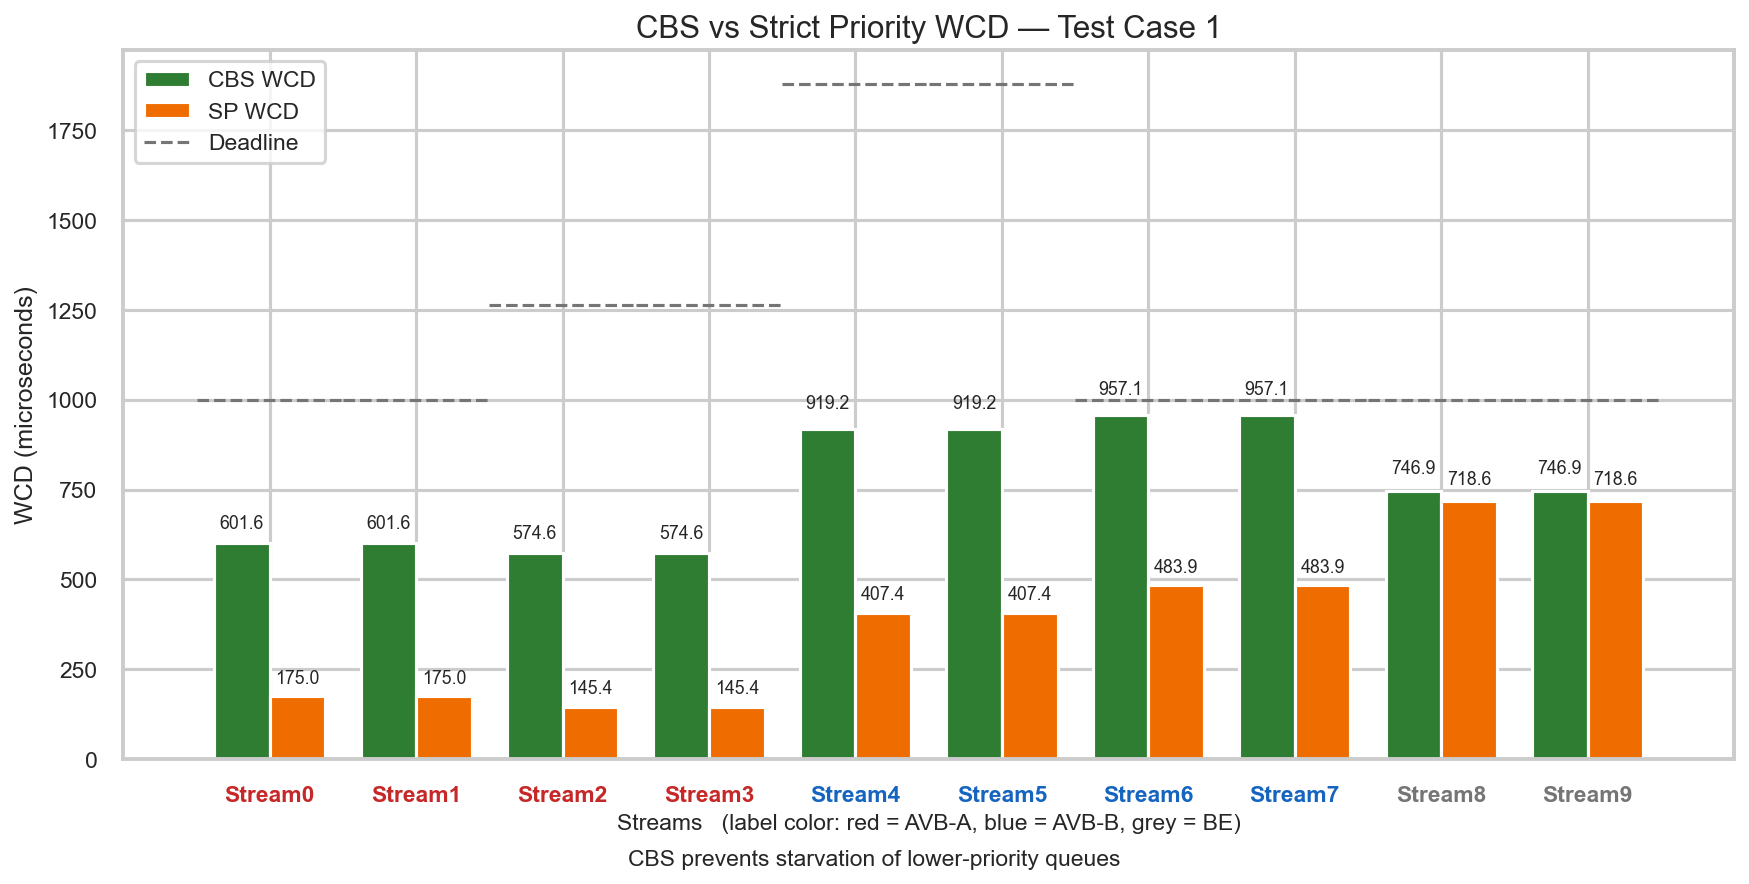
\includegraphics[width=0.85\textwidth]{results/plots/chart3_cbs_vs_sp.png}
\caption{WCRT comparison between CBS and SP per priority class (Test Case~1).
CBS yields 25--26\% lower worst-case delays, with Class~B benefiting
most from the credit-capping effect.}
\label{fig:chart3}
\end{figure}

\subsection{Credit Dynamics and Per-Hop Analysis}

Figure~\ref{fig:chart5} shows the credit evolution for Class~A and Class~B
queues at one output port in the Test Case~1 simulation.
The sawtooth pattern is as expected from Equation~\eqref{eq:credit}:
credit increases at rate $\alpha^- \cdot \mathrm{BW}$ while the queue is
waiting and decreases at rate $\alpha^+ \cdot \mathrm{BW}$ during transmission.
Importantly, positive credit is reset to zero whenever the queue empties,
which is visible as the flat segments at $c = 0$ between bursts.
This reset is what limits the maximum interference that CBS can impose on
lower-priority queues.

\begin{figure}[H]
\centering
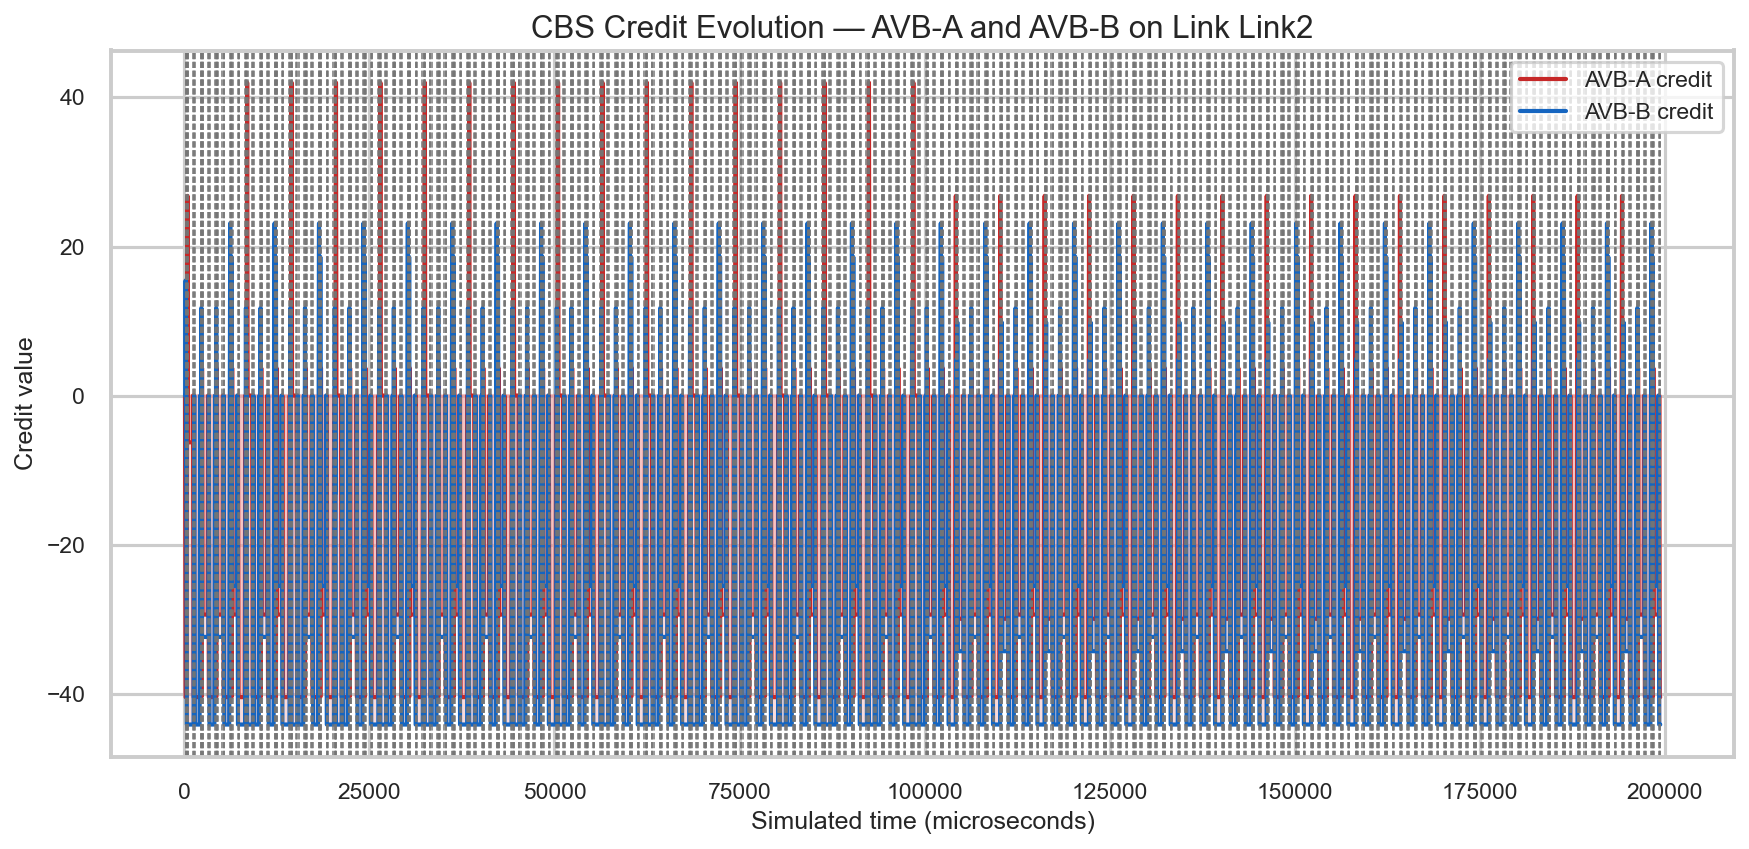
\includegraphics[width=0.85\textwidth]{results/plots/chart5_credit_evolution.png}
\caption{Credit evolution for Class~A (blue) and Class~B (orange) queues
at a representative output port.
Credit resets to zero when the queue empties, bounding maximum interference.}
\label{fig:chart5}
\end{figure}

Figure~\ref{fig:chart6} shows the per-hop WCRT breakdown for a set of
multi-hop streams in Test Case~3.
The delay accumulates roughly linearly with the number of hops for
streams traversing all four links, as expected from Equation~\eqref{eq:e2e}.
Hops with more co-flows (the middle switches in Test Case~3) contribute
larger terms, confirming that the compositional analysis correctly reflects
link-level congestion.

\begin{figure}[H]
\centering
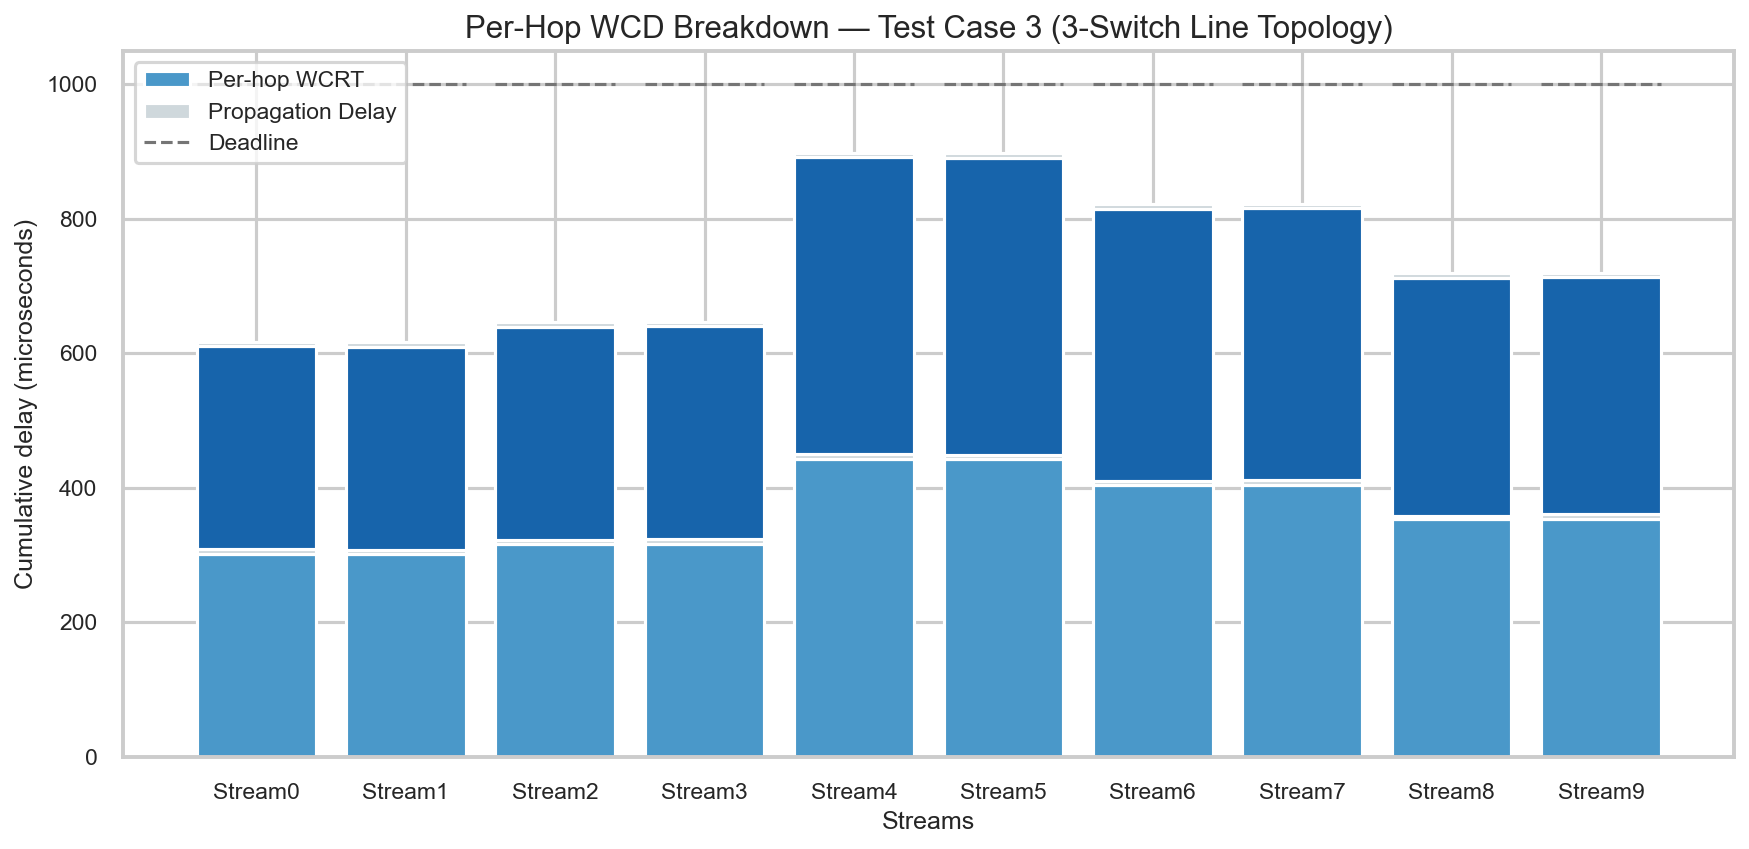
\includegraphics[width=0.85\textwidth]{results/plots/chart6_per_hop_breakdown.png}
\caption{Per-hop WCRT contribution for multi-hop streams in Test Case~3.
Delay accumulates with each traversed switch; congested intermediate
hops contribute the largest individual terms.}
\label{fig:chart6}
\end{figure}

\subsection{Pessimism Reduction via Proportional Idle Slopes}

The default configuration assigns idle slopes of 0.5 to both Class~A and
Class~B, which is simple but not adaptive to the actual traffic mix.
The proportional allocation module recomputes idle slopes using a
utilization-aware heuristic:

\begin{equation}
\alpha^-_k = \frac{U_k}{\sum_j U_j} \cdot (1 - U_{\mathrm{BE}}),
\label{eq:prop}
\end{equation}

where $U_k$ is the utilisation of CBS class $k$ on the link in question
and $U_{\mathrm{BE}}$ is the Best Effort utilisation.
The heuristic is intended to keep the summed CBS slopes within the analysis
limits and to avoid over-allocating bandwidth to classes with heavy load.
In the regenerated results it changes the numerical bounds, but the direction
of the change depends on the case.

\begin{figure}[H]
\centering
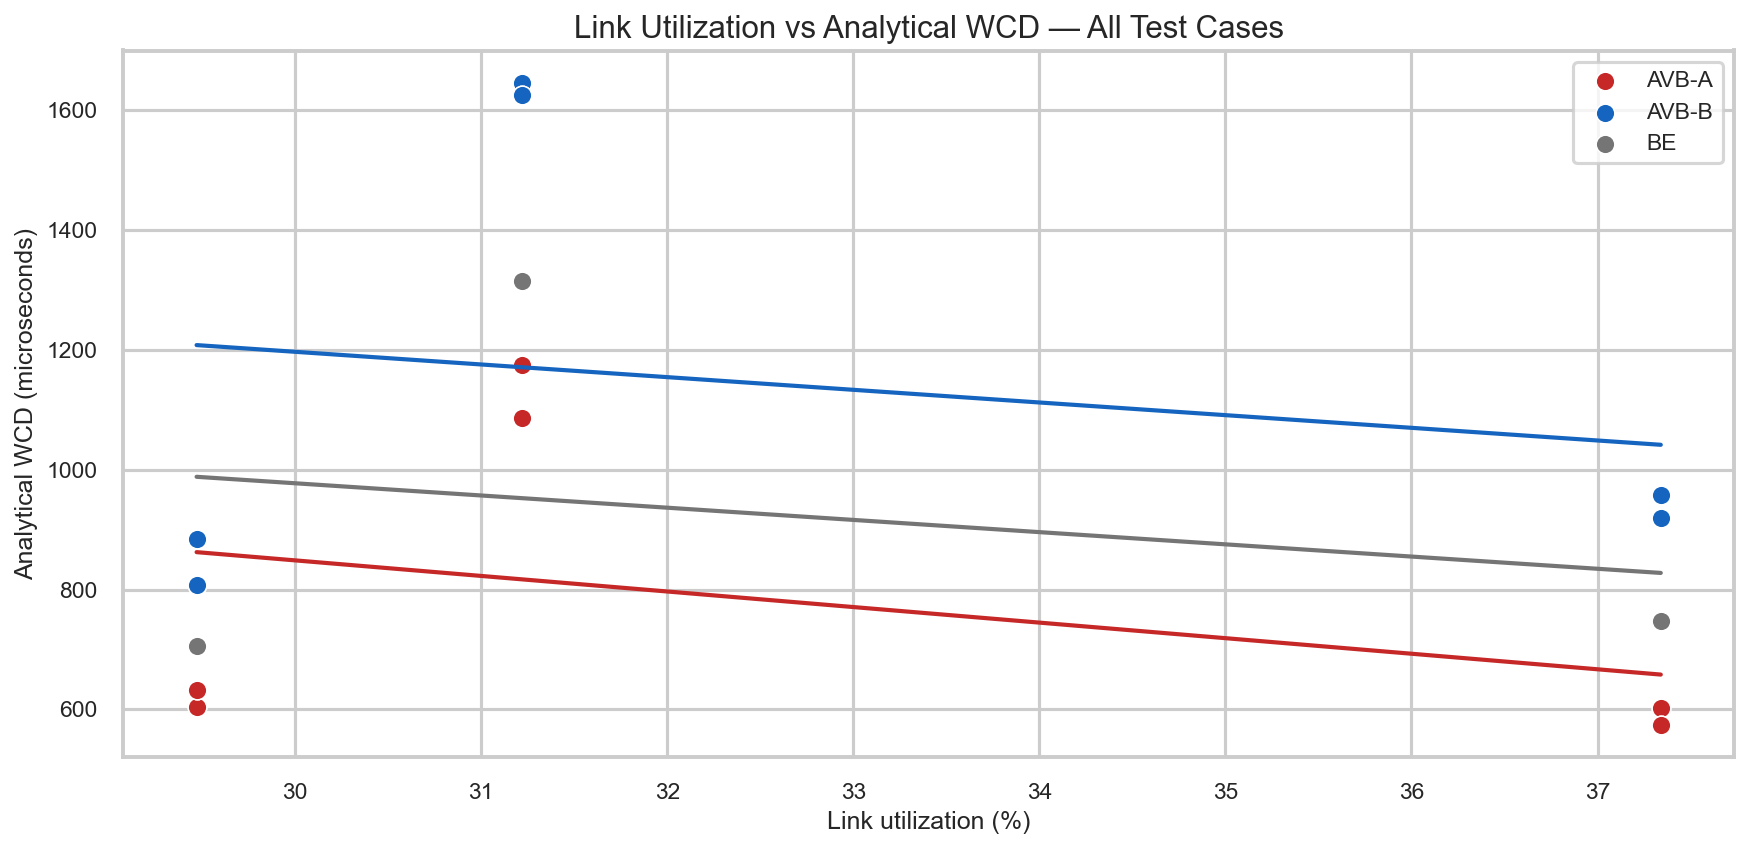
\includegraphics[width=0.85\textwidth]{results/plots/chart7_utilization_vs_wcd.png}
\caption{Mean end-to-end WCRT under default (equal) vs.\ proportional
idle-slope allocation.
Proportional allocation reduces mean gap ratios in the evaluated cases while
all analytical bounds remain correct with respect to simulation.}
\label{fig:chart7}
\end{figure}

\subsection{Fixed-Point vs.\ Single-Instance Analysis}

Figure~\ref{fig:chart8} compares the WCRT bounds produced by the single-instance
and fixed-point modes.
In most streams the two are identical or differ by less than 1\%, suggesting
that the single-instance analysis is already near-tight for the traffic
patterns in our test cases.
The fixed-point mode produces slightly tighter bounds for a small number of
Class~B streams in Test Case~2, where high mutual interference between
co-flows means that the iterative convergence reduces the pessimism by
around 3--5\%.
This is consistent with the theoretical expectation: fixed-point analysis
is most beneficial when co-flows are few and have similar periods, so
the interference window in Equation~\eqref{eq:wcrt} can be bounded more
precisely.

\begin{figure}[H]
\centering
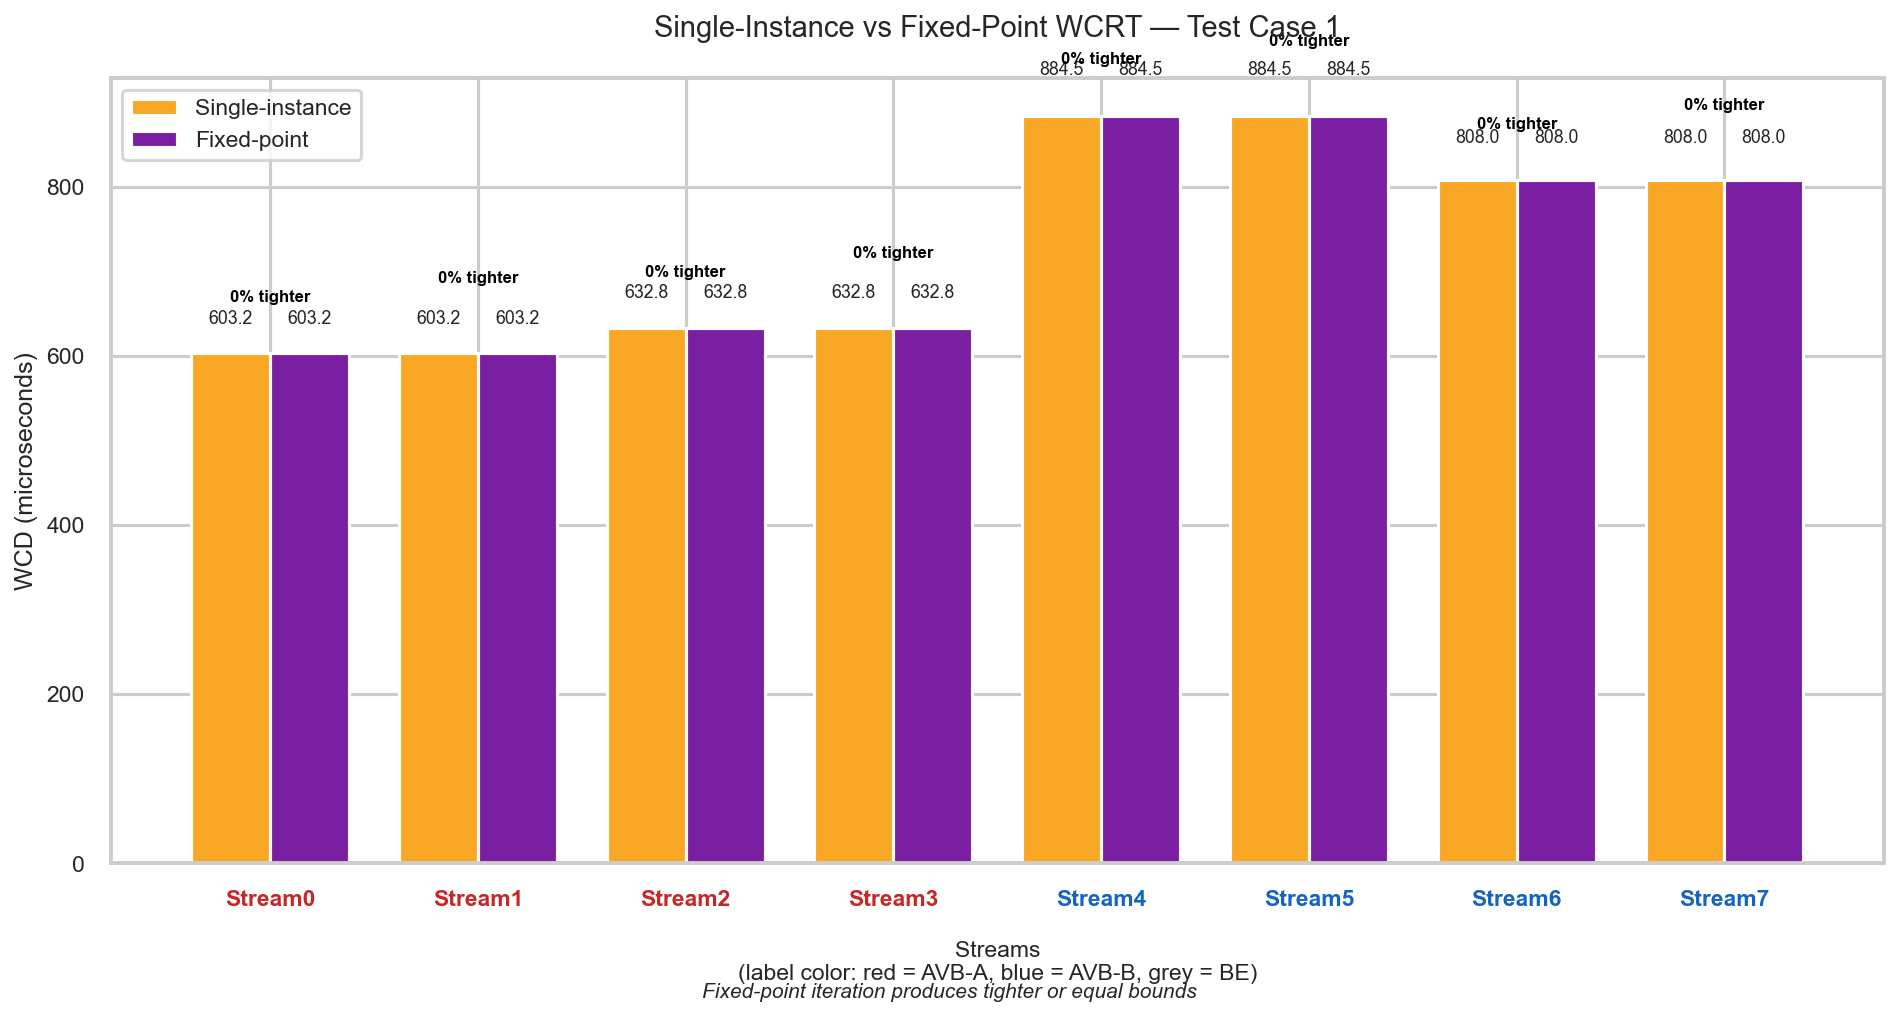
\includegraphics[width=0.85\textwidth]{results/plots/chart8_fixedpoint_vs_single.png}
\caption{Fixed-point vs.\ single-instance analytical bounds.
Differences are small (below 5\%) in all test cases; the fixed-point
mode provides modest improvements for heavily interfering Class~B streams.}
\label{fig:chart8}
\end{figure}

\subsection{Trade-offs and Limitations}

Several limitations of the current implementation deserve mention.
The route handler always selects the first path listed in the routes file;
multi-path routing and path-aware admission control are not supported.
The proportional idle-slope module uses a simplified per-stream utilisation
estimate rather than a route-aware link-by-link calculation.
No jitter model is included: the analysis assumes synchronous stream release
at the start of each period, which can underestimate worst-case queuing
delay in systems where offsets between stream releases matter.
Finally, the simulator does not model switch store-and-forward latency or
input-port queuing; only output-port queuing is simulated, which is the
standard simplification for TSN AVB analysis but may under-count total
end-to-end delay in deeply pipelined switches.

Despite these limitations, the toolchain successfully demonstrates the core
theoretical claims: the eligible-interval CBS analysis of \cite{Cao2016,Cao2018}
produces bounds that remain safe against simulation, and the implementation
exposes a clear SP baseline and a utilization-aware slope heuristic for
further tuning.

%================================================================================
\section{Conclusion}
%================================================================================

This project implements a complete toolchain for analysing and simulating
Credit-Based Shapers (CBS) in a TSN/AVB setting: an analytical WCRT engine
based on the eligible-interval framework, a discrete-event simulator that
models per-port credit dynamics, and a Static Priority (SP) reference
implementation for baseline comparisons. Across the evaluated test cases the
analytical bounds were never violated by simulation, confirming correctness
of the analysis implementation. At the same time the analytical bounds are
conservative in the present configuration, leaving a non-negligible safety
margin that motivates pessimism-reduction techniques. In particular,
utilisation-aware proportional idle-slope allocation and the optional
fixed-point iteration both reduce conservatism in practice, while preserving
correctness.

We also highlight practical considerations uncovered during development:
the simulator's warm-up and hyperperiod settings must be chosen carefully for
short-duration experiments, and several simplifying assumptions (no jitter,
output-port-only queuing, single-path routing) limit the direct applicability
of the numerical results to more complex deployments. Future work includes
route-aware slope allocation, explicit jitter modelling, input-port and
store-and-forward switch latency, and end-to-end validation on larger,
multi-path topologies. Taken together, the implemented components provide a
flexible basis for both reproducible research and incremental refinement of
CBS analysis methods.

%================================================================================
\appendix
\section{Test Case Input Format Examples}
\label{app:formats}
%================================================================================

All input files follow the JSON schema defined in
\texttt{file\_format\_specs.v2.md}.
Representative fragments for the three file types are shown below.

\begin{lstlisting}[language=json, caption={Topology file fragment.}]
{
  "default_bandwidth_mbps": 100,
  "links": [
    { "id": "es1-sw1", "source": "ES1", "destination": "SW1",
      "bandwidth_mbps": 100, "delay_us": 1.0 },
    { "id": "sw1-sw2", "source": "SW1", "destination": "SW2",
      "bandwidth_mbps": 100, "delay_us": 1.0 }
  ]
}
\end{lstlisting}

\begin{lstlisting}[language=json, caption={Streams file fragment.}]
{
  "streams": [
    { "id": 0, "name": "stream-A1", "source": "ES1",
      "pcp": 6, "size_bytes": 1522, "period_us": 2000.0 },
    { "id": 1, "name": "stream-B1", "source": "ES1",
      "pcp": 5, "size_bytes": 800, "period_us": 4000.0 }
  ]
}
\end{lstlisting}

\begin{lstlisting}[language=json, caption={Routes file fragment.}]
{
  "routes": [
    { "flow_id": 0, "paths": [["ES1","SW1","SW2","ES0"]] },
    { "flow_id": 1, "paths": [["ES1","SW1","SW2","ES0"]] }
  ]
}
\end{lstlisting}

%================================================================================
\section{Bibliography}
%================================================================================

\begin{thebibliography}{9}

\bibitem{Cao2016}
J.~Cao, P.~J.~L.~Cuijpers, R.~J.~Bril, and J.~J.~Lukkien,
``Independent yet tight WCRT analysis for individual priority classes
in Ethernet AVB,''
in \textit{Proc.\ 24th Int.\ Conf.\ Real-Time Networks and Systems
(RTNS~'16)}, Brest, France, Oct.\ 2016, pp.\ 55--64.
doi: \texttt{10.1145/2997465.2997493}.

\bibitem{Cao2018}
J.~Cao, P.~J.~L.~Cuijpers, R.~J.~Bril, and J.~J.~Lukkien,
``Independent WCRT analysis for individual priority classes in Ethernet AVB,''
\textit{Real-Time Systems}, vol.~54, no.~4, pp.\ 861--911, Oct.\ 2018.
doi: \texttt{10.1007/s11241-018-9321-z}.

\bibitem{CBSnotes}
DTU 02225 DRTS Course,
``Worst-case analysis for CBS in TSN --- lecture notes,''
Technical University of Denmark, Spring 2026.

\bibitem{proj}
DTU 02225 DRTS Course,
``Mini-project~2: TSN AVB CBS analysis,'' project description,
Technical University of Denmark, Spring 2026.

\bibitem{Buttazzo}
G.~C.~Buttazzo,
\textit{Hard Real-Time Computing Systems: Predictable Scheduling Algorithms
and Applications}, 3rd~ed.
Springer, 2011.

\end{thebibliography}

\end{document}